\section{Design and Implementation\label{design}}

\begin{figure}
\center
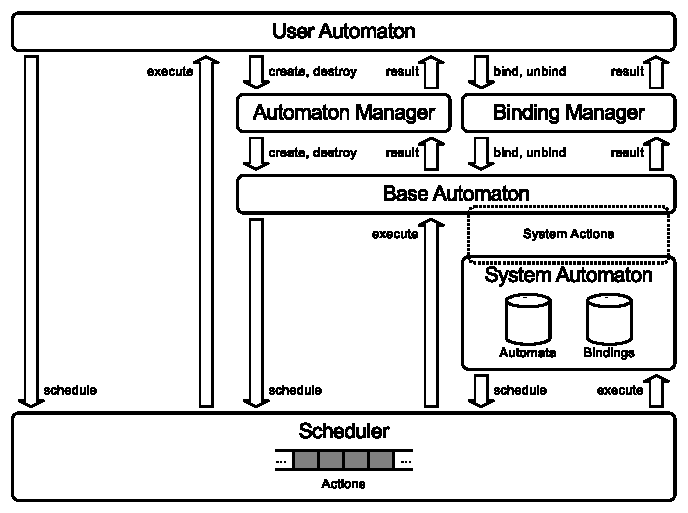
\includegraphics[width=.6\columnwidth]{architecture}
\caption{Framework architecture.}
\label{framework_architecture}
\end{figure}

The ioa++ framework is a C++ implementation of the component model described in Section~\ref{component_model} for POSIX environments.
The architecture of the ioa++ framework is depicted in Figure~\ref{framework_architecture}.

Conceptually, the set of automata $A$ and set of bindings $B$ belong to the system automaton.
However, the state they encode is shared and is used in the execution of every action.
A \emph{scheduler} uses $A$ to ensure that only actions belonging to automata that exist are selected and uses $B$ to ensure that the appropriate set of input actions receive the value produced when an output action is executed.
Thus, the set of actions implied by any action is the union of the set defined in Section~\ref{component_structure} and the system automaton.
The opportunities for concurrent execution discussed in Section~\ref{component_structure} hinge on the fact that \emph{only} actions that modify $A$ and $B$ must be serialized.
Binding predicates do not modify $B$ and therefore do not affect concurrent execution.
The scheduler is responsible for selecting and executing local actions subject to the I/O automata model and the concurrency constraints described in Section~\ref{component_model}.

All user automata inherit from a common base class (indicated by the Base Automaton layer shown in Figure~\ref{framework_architecture}) that provides facilities for asynchronously creating and destroying child automata and bindings.
The Base Automaton layer provides statically composed system actions that are used to communicate with the system automaton.
In most situations, the services provided by the Base Automaton layer are too low-level to be used directly by a user automaton.
Instead, an Automaton Manager provides a common higher-level interface for asynchronously managing a single child automaton using the services of the Base Automaton layer.
Similarly, a Binding Manager presents a high-level interface for asynchronously managing a single binding.

\subsection{Scheduler\label{scheduling}}

The scheduler is responsible for both selecting and executing local actions.
These two activities are decomposed into a \emph{dispatcher} that executes actions and a \emph{controller} that selects the next action.
The dispatcher enforces the execution and concurrency constraints of Section~\ref{component_model}.
Input actions are executed with corresponding output actions, according to the current set of bindings.
The dispatcher allows actions to be executed concurrently by (1)~requiring that the sets of automata implied by each action are disjoint and (2)~serializing all updates to the set of automata and bindings.
The controller encodes a \emph{policy} that selects the next local action.
For the framework to be a valid implementation of the I/O automata model, the controller used by the scheduler must be \emph{fair} as defined in Section~\ref{component_model}.
The run-time system can be initialized with different controllers to achieve different performance objectives.
The ioa++ framework distribution provides both a basic scheduler that is single-threaded and uses a single queue of actions that is processed using first-in/first-out semantics, and a multi-threaded scheduler with a configurable number of threads that we use in the performance evaluation described in Section~\ref{evaluation}.

\paragraph*{Explicit dynamic scheduling.}
In our framework implementation, automata to declare \emph{dynamically} the actions they would like the scheduler to consider.
%The act of declaring an action to the scheduler is called \emph{scheduling}.
Observe that executing an action potentially changes the state of the automaton and causes the set of enabled actions to change.
Consequently, an automaton is given the opportunity to declare actions to the scheduler (i.e., to \emph{schedule} them) after one of its actions is executed.
Since the state variables (and therefore preconditions) of all automata are independent, each automaton is responsible for scheduling its own actions.
For bootstrapping, each automaton is allowed to schedule actions when it is created.
Scheduling is idempotent to prevent unbounded growth of scheduler data structures.

\paragraph*{Binding predicates and scheduling.}
%% This assumption is not implicit because we state that the preconditions are independent.
The preceding discussion on scheduling assumed that an action in one automaton cannot affect preconditions in another automaton.
This is not entirely correct when one considers the system automaton and binding predicates.
For example, imagine an automaton with a single output action whose only precondition is that it must be bound and assume that the automaton only schedules the action when enabled.
When the automaton is created, its only action is disabled.
Consequently, it will not schedule its action and therefore will not be executed.
Suppose that some time after the automaton is created, another automaton successfully binds to the output action.
The bind action changes the precondition but the automaton will never be executed since it has no way of scheduling the output action.
While this example may seem contrived, it is representative of situations where an automaton is waiting for one or more of its outputs to be bound: a situation that occurs quite often in practice.
To remedy this, our framework takes advantage of the fair scheduling criteria of the I/O automata model and schedules an output action after each successful bind or unbind.

\paragraph*{Delayed actions.}
Scheduling activities for a future time is a useful feature for many systems because it allows the system to sleep between activities. For example, the framework should support the development of automata that act as timers and alarms.
Conceptually, an action is held until the time associated with it, at which point it is added to the set of actions being considered by the scheduler.
Actions scheduled in the past or present are released immediately to the scheduler.
When the same action is scheduled at two different times, the earliest time is used.
% Things I didn't say:  No canceling.

\paragraph*{File descriptor events.}
File descriptors are used to communicate with the outside world in a POSIX environment.
Observe that there is no concept of blocking in the I/O automata model and introducing blocking I/O operations into action effects may adversely affect the asynchronous and concurrent nature of I/O automata.
Thus, we require techniques that allow a program (1) to wait until a file descriptor is asynchronously ready for I/O and (2) to perform non-blocking I/O operations.
This implies the use of either the Proactor or Reactor pattern~\cite{schmidt2000pattern}.
The ioa++ framework uses the Reactor pattern since (1) it is simpler and (2) many operating systems have non-blocking I/O and some kind of synchronous I/O (de)multiplexing, whereas asynchronous I/O is less widespread.

Our use of the Reactor pattern causes an action to be scheduled when a file descriptor is ready for reading or writing.
A user automaton creates a file descriptor and configures it for non-blocking I/O.
The automaton then tells the scheduler to release an action (typically an internal action) whenever the automaton becomes ready for reading (or writing).
Subsequent requests made using the same file descriptor and event (ready for reading, ready for writing) are ignored.
Once the file descriptor is ready, the action is released for consideration by the controller.
The scheduler also provides a special function for closing file descriptors that purges them from the reactor.

\subsection{System Actions\label{system_action_section}}

Our approach to system actions follows the model introduced in Section~\ref{dynamics}.
All automata are statically composed with a system automaton via system actions for dynamically creating child automata, binding external actions, unbinding external actions, and destroying child automata.
The system automaton implements a request-response protocol where an automaton requests a system action and the system automaton processes the request and responds with an indication of either success or failure.
The protocol used by automata to asynchronously manage child automata and bindings is suitable for simple constellations but becomes unwieldy when creating more complicated ones.
Automaton Managers and Binding Managers provide individualized facades to the system action state machines.
Creating an Automaton Manager initiates the creation of a new child automaton and invoking a destroy method initiates the destruction of a child automaton.
Automaton Managers can be monitored using the Observer~\cite{gamma1995design} pattern to determine when and how the creation/destruction process succeeds.
Binding Managers are similar except they do not begin the process of binding until the automata providing the output action and input action have been created: thus, Binding Managers observe Automaton Managers.

\ifjournal
\paragraph*{Generators.}
A \emph{generator} is a single-use factory for creating an instance of an automaton.
Generators are used to produce new automata as part of the create system action and are visible as arguments in the various layers of the framework.
\fi
